\documentclass[a4paper,12pt]{article}

% \usepackage[latin1]{inputenc}
\usepackage[utf8]{inputenc} 
\usepackage[italian]{babel}
\usepackage{indentfirst}
\usepackage[margin=2.2cm]{geometry}
\usepackage[most]{tcolorbox}
\usepackage{graphicx}
\usepackage{hyperref}
\usepackage[italian]{varioref}
\usepackage{listings}
\usepackage{xcolor}
\usepackage[numbered,framed]{matlab-prettifier}
\usepackage[font={small}]{caption}

\usepackage{tikz}
\usetikzlibrary{positioning}
\tikzset{%
  every neuron/.style={
    circle,
    draw,
    minimum size=1cm
  },
  neuron missing/.style={
    draw=none, 
    scale=4,
    text height=0.333cm,
    execute at begin node=\color{black}$\vdots$
  },
}

\captionsetup[figure]{labelfont={bf},name={Figura},labelsep=period}

\renewcommand*{\fullref}[1]{\hyperref[{#1}]{\vref*{#1}, \emph{\nameref*{#1}}}}
\newcommand*{\coderef}[1]{\hyperref[{#1}]{\nameref*{#1} a pagina \pageref*{#1}}}

\renewcommand{\textfraction}{0.05}
\renewcommand{\topfraction}{0.9}
\renewcommand{\bottomfraction}{0.9}
\renewcommand{\floatpagefraction}{0.8}

\graphicspath{{figures/}}


\title{\textbf{MNIST – Rete Neurale per il Riconoscimento di Cifre Manoscritte}}
\author{Lara Vignotto}
\date{\today}  


\begin{document}

\maketitle
% \vspace{.5cm}
\vfill
\tableofcontents
% \vspace{5cm}


\newpage
% \setcounter{section}{-1}
%%%%%%%%%%%%%%%%%%%%%%%%%%%%%%
\section{Presentazione e scopi del progetto}
Lo scopo di questo progetto è la realizzazione, l'analisi e la documentazione di una rete neurale per la classificazione delle dieci cifre $0-9$ scritte a mano provenienti dal dataset MNIST. Ogni immagine ha
dimensione $28\times28$ pixel ed è rappresentata in scala di grigi. Il lavoro è diviso nelle seguenti sezioni:
\begin{itemize}
    \item Nel \textbf{secondo capitolo} presenteremo le specifiche del modello di rete neurale adottato e l'architettura che ne deriva;
    \item Il \textbf{terzo capitolo} è dedicato alla preparazione dei dati;
    \item Nel \textbf{quarto capitolo} daremo un'architettura del software: svilupperemo le fasi di apprendimento e la progettazione generale della rete;
    \item Nel \textbf{quinto capitolo} illustreremo la prima procedura del pacchetto, relativa alla preparazione degli insiemi di dati;
    \item Il \textbf{sesto capitolo} sarà dedicato alla seconda procedura, che implementa la strutturazione della rete e la fase di apprendimento;
    \item Nel \textbf{settimo capitolo} presenteremo i risultati;
    \item Nell'\textbf{ottavo capitolo} discuteremo i risultati riportati al capitolo precedente.
\end{itemize}

\vfill
\hfill Lara Vignotto

\hfill \today




\newpage
%%%%%%%%%%%%%%%%%%%%%%%%%%%%%%
\section{Modello e architettura della rete} % cap2

La rete neurale è composta da tre strati (Figura~\vref{fig:modello}):
\begin{itemize}
    \item Un \emph{input layer} di 784 nodi, che corrispondono ai $28\times28$ pixel di ciascuna immagine;
    \item Un \emph{hidden layer} di 30 nodi con funzione di attivazione ReLU;
    \item Un \emph{output layer} di 10 nodi con funzione di attivazione Softmax, uno per ogni categoria o classe, ovvero le cifre $0-9$.
\end{itemize}

\begin{figure}[htb]
    \centering
    \tcbox[boxrule=.3mm,colback=white]{
% tikz picture from
% https://tex.stackexchange.com/a/153974
\begin{tikzpicture}[x=2cm, y=1.5cm, >=stealth]

    \foreach \m/\l [count=\y] in {1,2,3,missing,4}
    \node [every neuron/.try, neuron \m/.try] (input-\m) at (0,2.5-\y) {};

    \foreach \m [count=\y] in {1,missing,2}
    \node [every neuron/.try, neuron \m/.try ] (hidden-\m) at (2,2-\y*1.25) {};

    \foreach \m [count=\y] in {1,missing,2}
    \node [every neuron/.try, neuron \m/.try ] (output-\m) at (4,1.5-\y) {};

    \foreach \l [count=\i] in {1,2,3,784}
    \draw [<-] (input-\i) -- ++(-1,0)
        node [above, midway] {$I_{\l}$};

    \foreach \l [count=\i] in {1,30}
    \node [] at (hidden-\i) {$H_{\l}$};

    \foreach \l [count=\i] in {1,10}
    \draw [->] (output-\i) -- ++(1,0)
        node [above, midway] {$O_{\l}$};

    \foreach \i in {1,...,4}
    \foreach \j in {1,...,2}
        \draw [->] (input-\i) -- (hidden-\j);

    \foreach \i in {1,...,2}
    \foreach \j in {1,...,2}
        \draw [->] (hidden-\i) -- (output-\j);

    \foreach \l [count=\x from 0] in {Input, Hidden, Ouput}
    \node [align=center, above] at (\x*2,2) {\l \\ layer};

\end{tikzpicture}
    }
    \caption{Schema della rete neurale.}\label{fig:modello}
\end{figure}




\newpage
%%%%%%%%%%%%%%%%%%%%%%%%%%%%%%
\section{Preparazione dei dati} % cap3


%%%%%%%%%%%%%
\subsection{Il database MNIST}
MNIST è un database di 70 000 immagini in scala di grigi di cifre scritte a mano. È diviso in una partizione di apprendimento di 60 000 immagini e una partizione di test di 10 000 immagini. Ogni cifra è stata normalizzata in base alle dimensioni, e centrata in un'immagine con una risoluzione di $28\times28$ pixel. Ad ogni immagine è associata un'etichetta (\emph{label}) che denota quale cifra da 0 a 9 l'immagine rappresenta. 


%%%%%%%%%%%%%
\subsection{Lo splitting}
Decidiamo di partizionare il dataset MNIST in due insiemi: il \emph{training set} per l'apprendimento e il \emph{validation set} per la valutazione delle prestazioni della rete.
\begin{itemize}
    \item \emph{Training set}: insieme di coppie di array (\emph{input}, \emph{output}) usate per addestrare la rete, ovvero per modificare i pesi delle connessioni. In questo progetto il \emph{training set} equivale all'insieme delle coppie \texttt{(immagine; cifra rappresentata)};
    \item \emph{Validation set}: insieme di coppie di array (\emph{input}, \emph{output}) per la verifica dell'apprendimento della rete. Lo utilizzeremo in parallelo per monitorare l'apprendimento durante il suo svolgersi e, al termine, valutarne le prestazioni. Comprende anche stimoli che non sono stati usati in fase di apprendimento.
\end{itemize}

Si usa spesso un ulteriore insieme, il \emph{testing set}, insieme di istanze a cui non è associato l'output corretto. È l'insieme delle istanze non usate per l'apprendimento e date in input alla rete addestrata per verificane la capacità di generalizzazione.





\newpage
%%%%%%%%%%%%%%%%%%%%%%%%%%%%%%
\section{Struttura del software} % cap4
Il pacchetto per la rete neurale per il riconoscimento di cifre scritte a mano è articolato nei seguenti due moduli:
\begin{itemize}
    \item La funzione \texttt{MNIST\_DataPrep} per la preparazione dei dati. Dato in input un valore \texttt{p} compreso tra 0 e 1, carica le immagini dal dataset MNIST ed esegue lo \emph{splitting} dello stesso in due insiemi. Restituisce gli insiemi, il primo contenente una percentuale di elementi del dataset pari a \texttt{p}, l'altro contenente i restanti elementi;
    \item Lo script \texttt{MNIST\_Training} per la definizione dell'architettura di rete, la fase di apprendimento e la fase di verifica. Richiama la funzione \texttt{MNIST\_DataPrep} per costruire il \emph{training set} e il \emph{validation set}. Definisce l'architettura della rete, ovvero gli strati di cui è composta, il numero di nodi per ogni strato, e le funzioni di attivazione utilizzate. Successivamente implementa la fase di addestramento della rete, specificando delle opzioni di apprendimento. Infine viene valutata l'accuratezza della validazione.
\end{itemize}





\newpage
%%%%%%%%%%%%%%%%%%%%%%%%%%%%%%
\section{La procedura \texttt{MNIST\_DataPrep}} % cap5

\begin{lstlisting}[style=Matlab-editor,title=\texttt{MNIST\_DataPrep.m},label=lst:dataprep]
function [imds1, imds2] = MNIST_DataPrep(p)
%   Caricamento delle immagini da MNIST
    digitDatasetPath = fullfile(matlabroot,'toolbox', ...
        'nnet','nndemos','nndatasets','DigitDataset');
    imds = imageDatastore(digitDatasetPath, ... 
        'IncludeSubFolders',true,'LabelSource','foldernames');
%
%   Visualizzazione di un insieme casuale delle immagini
    figure
    perm = randperm(10000,20);
%
    for i = 1:20
        subplot(4, 5, i);
        imshow(imds.Files{perm(i)});
    end
%
%   Splitting
    [imds1,imds2] = splitEachLabel(imds,p,'randomized');
end
\end{lstlisting}

\subsection{Caricamento dei dati MNIST e visualizzazione.} La funzione definisce il \texttt{di\-gi\-tal\-Da\-ta\-set\-Path}, ovvero il percorso assoluto alla cartella contenente i dati che ci servono. Carica poi le istanze di cifre come \texttt{imageDatastore} in \texttt{imds}.

Abbiamo visualizzato 20 immagini estratte a caso dal datastore di 10 000 immagini usando la procedura \texttt{randperm()} (Figura~\vref{fig:a3}).

\begin{figure}[htb]
    \centering
    \tcbox[boxrule=.3mm,colback=white]{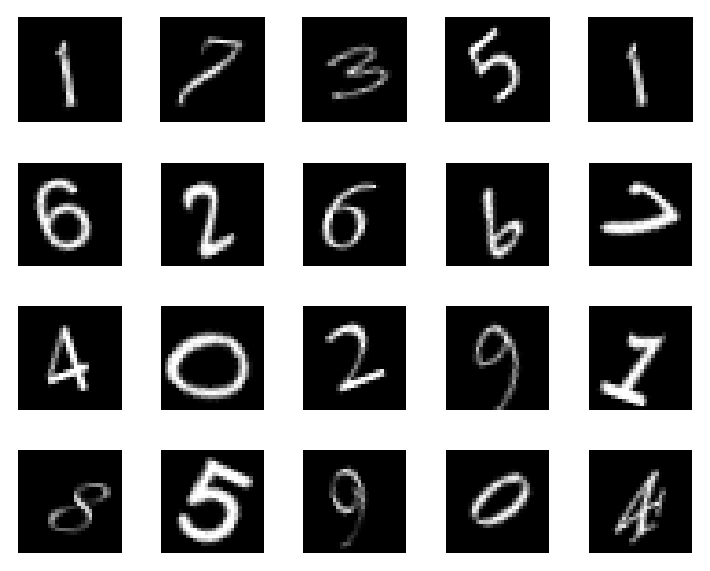
\includegraphics[width=.58\textwidth]{fig-a3.eps}}
    \caption{Venti immagini casuali di cifre dal dataset MNIST.}
    \label{fig:a3}
\end{figure}

\subsection{Splitting.} La funzione, infine, effettua lo splitting, ovvero divide il dataset \texttt{imds} in \emph{training set} e \emph{validation set}. In particolare, come vedremo nello script successivo, stabiliremo una proporzione di $0.8$ (specificando \texttt{p}) tra le cardinalità dei due insiemi.

Abbiamo visualizzato a schermo le caratteristiche dei due insiemi appena creati, che abbiamo chiamato \texttt{imdsTrain} e \texttt{imdsValidation}. Il primo contiene 8000 \emph{samples}, mentre il secondo ne contiene 2000: sono rispettate le proporzioni di $0.8$.
\begin{lstlisting}[style=Matlab-editor,title=\texttt{imdsTrain},label=lst:imdsTrain]
imdsTrain = 

  ImageDatastore with properties:

                       Files: {
                              ' ...\R2020b\toolbox\nnet\nndemos\nndatasets\DigitDataset\0\image9001.png';
                              ' ...\R2020b\toolbox\nnet\nndemos\nndatasets\DigitDataset\0\image9004.png';
                              ' ...\R2020b\toolbox\nnet\nndemos\nndatasets\DigitDataset\0\image9005.png'
                               ... and 7997 more
                              }
                     Folders: {
                              ' ...\MATLAB\R2020b\toolbox\nnet\nndemos\nndatasets\DigitDataset'
                              }
                      Labels: [0; 0; 0 ... and 7997 more categorical]
    AlternateFileSystemRoots: {}
                    ReadSize: 1
      SupportedOutputFormats: ["png"    "jpg"    "jpeg"    "tif"    "tiff"]
         DefaultOutputFormat: "png"
                     ReadFcn: @readDatastoreImage
\end{lstlisting}

\begin{lstlisting}[style=Matlab-editor,title=\texttt{imdsValidation},label=lst:imdsValidation]
imdsValidation = 

  ImageDatastore with properties:

                       Files: {
                              ' ...\R2020b\toolbox\nnet\nndemos\nndatasets\DigitDataset\0\image10000.png';
                              ' ...\R2020b\toolbox\nnet\nndemos\nndatasets\DigitDataset\0\image9002.png';
                              ' ...\R2020b\toolbox\nnet\nndemos\nndatasets\DigitDataset\0\image9003.png'
                               ... and 1997 more
                              }
                     Folders: {
                              ' ...\MATLAB\R2020b\toolbox\nnet\nndemos\nndatasets\DigitDataset'
                              }
                      Labels: [0; 0; 0 ... and 1997 more categorical]
    AlternateFileSystemRoots: {}
                    ReadSize: 1
      SupportedOutputFormats: ["png"    "jpg"    "jpeg"    "tif"    "tiff"]
         DefaultOutputFormat: "png"
                     ReadFcn: @readDatastoreImage
\end{lstlisting}


\newpage
%%%%%%%%%%%%%%%%%%%%%%%%%%%%%%
\section{La procedura \texttt{MNIST\_Training}} % cap6

\begin{lstlisting}[style=Matlab-editor,title=\texttt{MNIST\_Training.m},label=lst:training]
[imdsTrain, imdsValidation] = MNIST_DataPrep(0.8);
%
layers = [ ...
    imageInputLayer([28 28 1],'Name','input')

    fullyConnectedLayer(30,'Name','hidden_layer_1')
    batchNormalizationLayer('Name','BN_1')
    reluLayer('Name','relu')
   
    fullyConnectedLayer(10,'Name','output_layer')
    softmaxLayer('Name','softmax')
    classificationLayer('Name','classOutput')];
%
%%%%%%%%%%%%%%% Apprendimento
%
% Specifica delle opzioni di apprendimento
options = trainingOptions( ...
    'sgdm', ...
    'InitialLearnRate',0.01, ...
    'MaxEpochs',8, ...
    'Shuffle','every-epoch', ...
    'ValidationData',imdsValidation, ...
    'ValidationFrequency',30, ...
    'Verbose',false, ...
    'Plots','training-progress');
%
% Apprendimento usando il training set
[net,info] = trainNetwork(imdsTrain,layers,options);
%
% Analizza l'architettura di rete
analyzeNetwork(net)
%
%%%%%%%%%%%%%%% Validazione
YPred = classify(net,imdsValidation);
YValidation = imdsValidation.Labels;
%
% Accuratezza della validazione
accuracy = sum(YPred == YValidation)/numel(YValidation)
%
% Memorizzazione su file
save('MNIST_NeuralNet.mat','info');
\end{lstlisting}


\subsection{Definizione della struttura di rete}
Lo script richiama la funzione \texttt{MNIST\_DataPrep} per la creazione di \texttt{imdsTrain} (\emph{training set}) e \texttt{imdsValidation} (\emph{validation set}).

Con l'istruzione \texttt{layers} costruisce la rete neurale strato per strato, definendone l'architettura. In particolare, gli strati utilizzati sono:
\begin{itemize}
    \item \texttt{imageInputLayer}: è stata specificata la dimensione delle immagini di input, ovvero $28\times28$;
    \item \texttt{fullyConnectedLayer}: strato in cui i neuroni si connettono a tutti i neuroni dello strato precedente;
    \item \texttt{batchNormalizationLayer}: lo strato \emph{batch normalization} normalizza le attivazioni e i gradienti che si propagano attraverso una rete. 
    
    Applicando la \emph{batch normalization} a uno strato della rete, vengono normalizzati gli \emph{output} della funzione di attivazione relativa a quello strato, ovvero gli \emph{input} del \emph{batch normalization layer}. La normalizzazione di questi valori $x_i$ avviene calcolando dapprima la media $\mu_B$ e la varianza $\sigma^2_B$ su un mini-batch e su ogni canale di \emph{input}, e successivamente calcolando le attivazioni normalizzate come 
    \[
        \widehat{x_i} = \dfrac{x_i-\mu_B}{\sqrt{\sigma^2_B+\epsilon}}  
    \]
    Questo fa in modo che gli \emph{input} abbiano media uguale a 0 e varianza pari a 1, ovvero che siano normalizzati. Nel caso in cui questi valori non siano ottimali per lo strato successivo, il \emph{batch normalization layer} ridimensiona ulteriormente le attivazioni come
    \[
        y_i = \gamma\widehat{x_i} + \beta       
    \]
    I valori di media, varianza, $\beta$ e $\gamma$ sono tutti ``addestrabili'', cioé vengono tutti ottimizzati durante la fase di apprendimento.

     Questo processo riduce le fluttuazioni nel calcolo dei pesi in fase di apprendimento, impedendo che i valori dei pesi diventino estremamente alti o bassi. Il risultato dei calcoli effettuati dallo strato \emph{batch normalization} è quindi una stabilizzazione dei pesi della rete;
    \item \texttt{reluLayer}: funzione di attivazione ReLU;
    \item \texttt{softmaxLayer}: funzione di attivazione Softmax;
    \item \texttt{classificationLayer}: il \emph{classification layer} utilizza gli \emph{output} restituiti dalla funzione di attivazione softmax, ovvero delle probabilità (che l'\emph{output} sia classificato correttamente), e calcola una misura delle prestazioni della rete, la \emph{cross entropy loss}. In questo lavoro utilizziamo questa funzione come stima della prestazione della rete, invece che la funzione \emph{loss} calcolata con gli MSE, in quanto la rete ha carattere statistico: abbiamo una classificazione tra 10 categorie (le cifre da 0 a 9). Essendo questa funzione una \emph{loss}, ci aspettiamo che il processo di apprendimento porti a una sua diminuzione.
    
    Nel \emph{classification layer} vengono presi i valori dalla funzione softmax e ogni \emph{input} viene assegnato ad una delle $K$ classi che si escludono a vicenda utilizzando la funzione \emph{cross entropy}:
    \[
        \text{loss} = -\sum_{i=1}^N\sum_{j=1}^N t_{ij} \ln y_{ij}    
    \]
    dove $N$ è il numero di $samples$, $K$ è il numero di classi, $t_{ij}$ è l'indicatore che l'$i$-esimo campione appartiene alla $j$-esima classe, e $y_{ij}$ è l'output del campione $i$ per la classe $j$ (in questo caso il valore dalla funzione softmax), ovvero la probabilità che la rete associ l'$i$-esimo \emph{input} con la classe $j$.
\end{itemize}

È stata effettuata la verifica della struttura della rete utilizzando la procedura \texttt{analyzeNetwork()}. Lo schema di sintesi è riportato in Figura~\vref{fig:6a3}.

\begin{figure}[htb]
    \hspace*{-3cm}\framebox{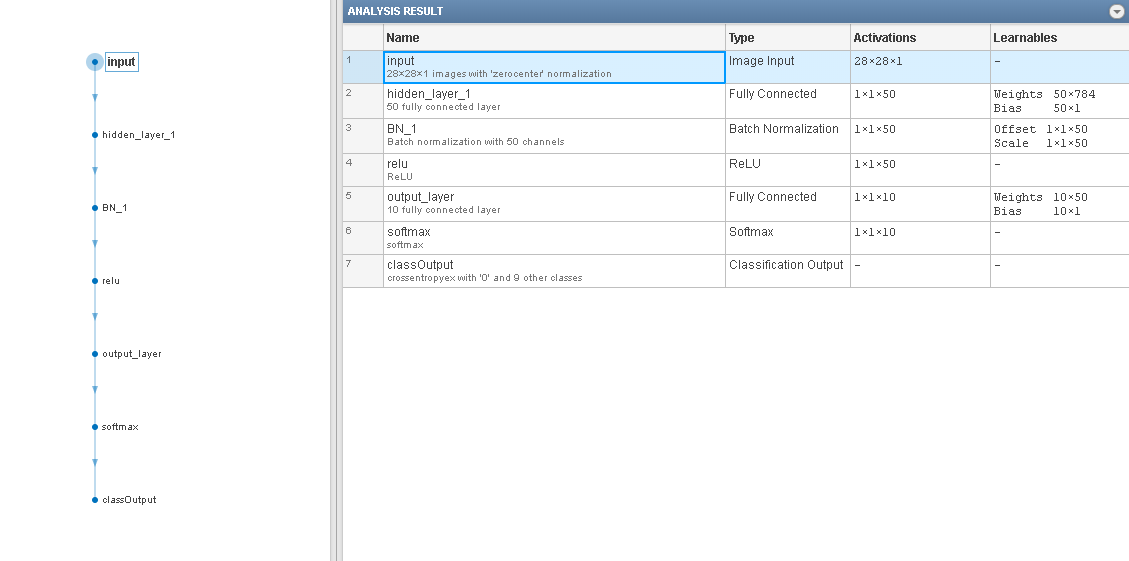
\includegraphics[width=1.3\textwidth]{fig-6a3.png}}
    \caption{Modello di rete neurale multistrato.}
    \label{fig:6a3}
\end{figure}




\subsection{Fase di apprendimento}\label{sec:fase-apprendimento}
La fase di addestramento della rete inizia con la definizione delle opzioni di apprendimento. Questa specifica viene eseguita con l'istruzione \texttt{trainingOptions}. la rete viene addestrata utilizzando lo \emph{stochastic gradient descent with momentum}, con un tasso di apprendimento iniziale di $0.01$. Il numero massimo di epoche è impostato a 8. Specificando \texttt{ValidationData} e \texttt{ValidationFrequency} viene monitorata l'accuratezza della rete, ovvero viene calcolata l'accuratezza sui dati di validazione a intervalli regolari durante l'apprendimento. Analizziamo in particolare due opzioni:

\begin{itemize}
    \item \texttt{sgdm}: L'algoritmo di \emph{stochastic gradient descent} aggiorna i valori dei pesi per ridurre al minimo la funzione \emph{loss} compiendo piccoli passi ad ogni iterazione nella direzione del gradiente negativo della \emph{loss}. Ad ogni iterazione questo algoritmo valuta il gradiente e aggiorna i pesi utilizzando un sottoinsieme (mini-batch) dei dati di addestramento, a differenza dell'algoritmo standard di discesa lungo il gradiente, che valuta il gradiente della \emph{loss function} utilizzando l'intero \emph{training set}. Ad ogni iterazione viene utilizzato un mini-batch diverso, e il passaggio completo dell'algoritmo di addestramento sull'intero \emph{training set} utilizzando i mini-batch è un'epoca. La discesa del gradiente è stocastica perché gli aggiornamenti dei pesi calcolati utilizzando un mini-batch sono una stima rumorosa dell'aggiornamento dei pesi che risulterebbe dall'utilizzo dell'intero set di dati. 
    
    L'algoritmo di \emph{stochastic gradient descent} può oscillare lungo il percorso di discesa verso l'ottimale: per ridurre questa instabilità numerica si può aggiungere un termine \emph{momentum} all'aggiornamento dei pesi. La tecnica algoritmica dello \emph{stochastic gradient descent with momentum} è quindi una variazione dell'algoritmo di discesa lungo il gradiente che permette di operare una stabilizzazione;
    \item \texttt{Shuffle}: è l'opzione per ``mescolare'' i dati. \texttt{every-epoch} mescola il \emph{training set} prima di ogni epoca di addestramento, e mescola il \emph{validation set} prima di ogni validazione.
\end{itemize}

L'apprendimento vero e proprio avviene sul \emph{training set} tramite la procedura \texttt{tra\-in\-Net\-work()}. Questa procedura istanzia l'oggetto \texttt{net}:

\begin{lstlisting}[style=Matlab-editor,label=lst:net]
net = 

  SeriesNetwork with properties:

         Layers: [7x1 nnet.cnn.layer.Layer]
     InputNames: {'input'}
    OutputNames: {'classOutput'}
\end{lstlisting}

Un oggetto \texttt{SeriesNetwork} è una rete neurale per il deep learning con strati disposti uno dopo l'altro. Ha un unico strato di \emph{input} e un unico stato di \emph{output}.\medskip

Lo script, infine, esegue la validazione dell'apprendimento utilizzando il \texttt{validation set} nella procedura \texttt{classify()}. Calcola in seguito l'accuratezza finale della validazione, ossia la frazione di etichette che la rete classifica correttamente.



\newpage
%%%%%%%%%%%%%%%%%%%%%%%%%%%%%%
\section{Risultati} % cap7

\subsection{Curva di apprendimento della rete}
Eseguendo lo script \texttt{MNIST\_Training} si ottiene la curva di apprendimento in Figura~\vref{fig:training}. La \emph{validation accuracy} è $92.90\%$.

\begin{figure}[htb]
    \hspace*{-2.1cm}\framebox{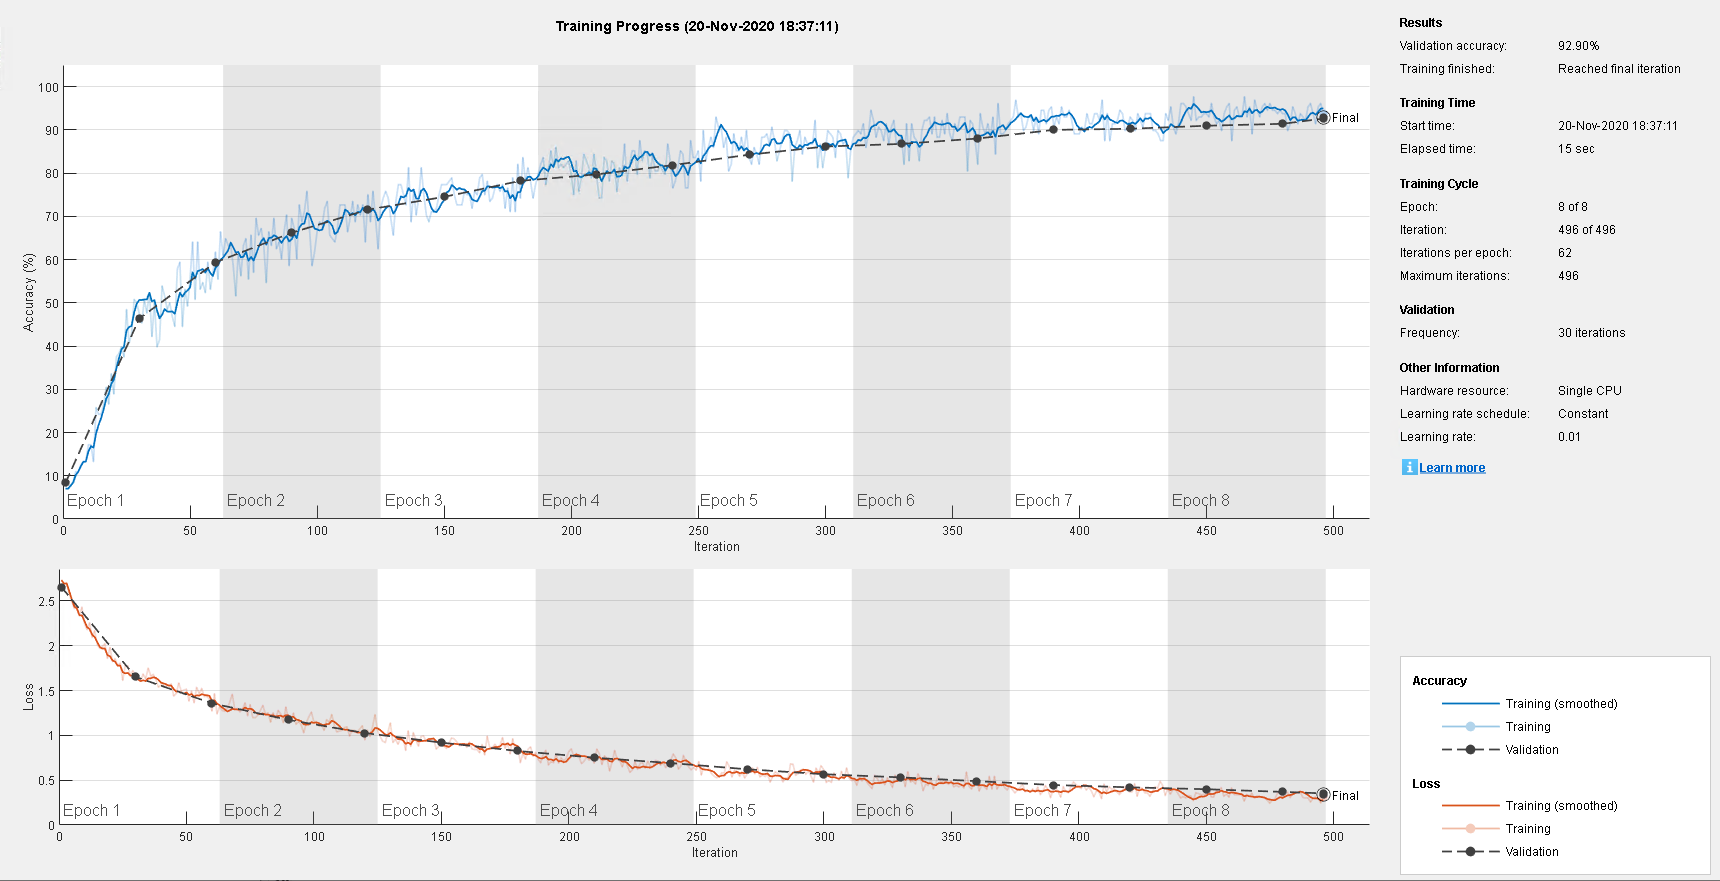
\includegraphics[width=1.24\textwidth]{fig-training.png}}
    \caption{Curva di apprendimento della rete.}
    \label{fig:training}
\end{figure}



\subsection{Validazione dell'apprendimento}
Come visto nella sezione \fullref{sec:fase-apprendimento}, al termine dello script \texttt{MNIST\_Training} abbiamo effettuato la validazione dell'apprendimento calcolando l'accuratezza finale della validazione:
\begin{lstlisting}[style=Matlab-editor,label=lst:accuracy]
accuracy =

    0.9105
\end{lstlisting}
 


\newpage
\subsection{Curve di apprendimento al variare della percentuale di partizione del dataset}
Abbiamo effettuato tre distinte partizioni del datastore secondo tre percentuali tra le cardinalità del \emph{training set} e del \emph{validation set}: $0.4$, $0.75$, $0.9$. Le curve di apprendimento risultanti sono riportate nelle Figure~\vref{fig:04},~\vref{fig:075} e~\vref{fig:09}.\medskip

Le \emph{validation accuracy} sono:
\begin{itemize}
    \item Percentuale \emph{training}/\emph{validation} $0.4$: $81.63\%$;
    \item Percentuale \emph{training}/\emph{validation} $0.75$: $90.00\%$;
    \item Percentuale \emph{training}/\emph{validation} $0.9$: $93.40\%$.
\end{itemize}

\begin{figure}[htb]
    \hspace*{-2.1cm}\framebox{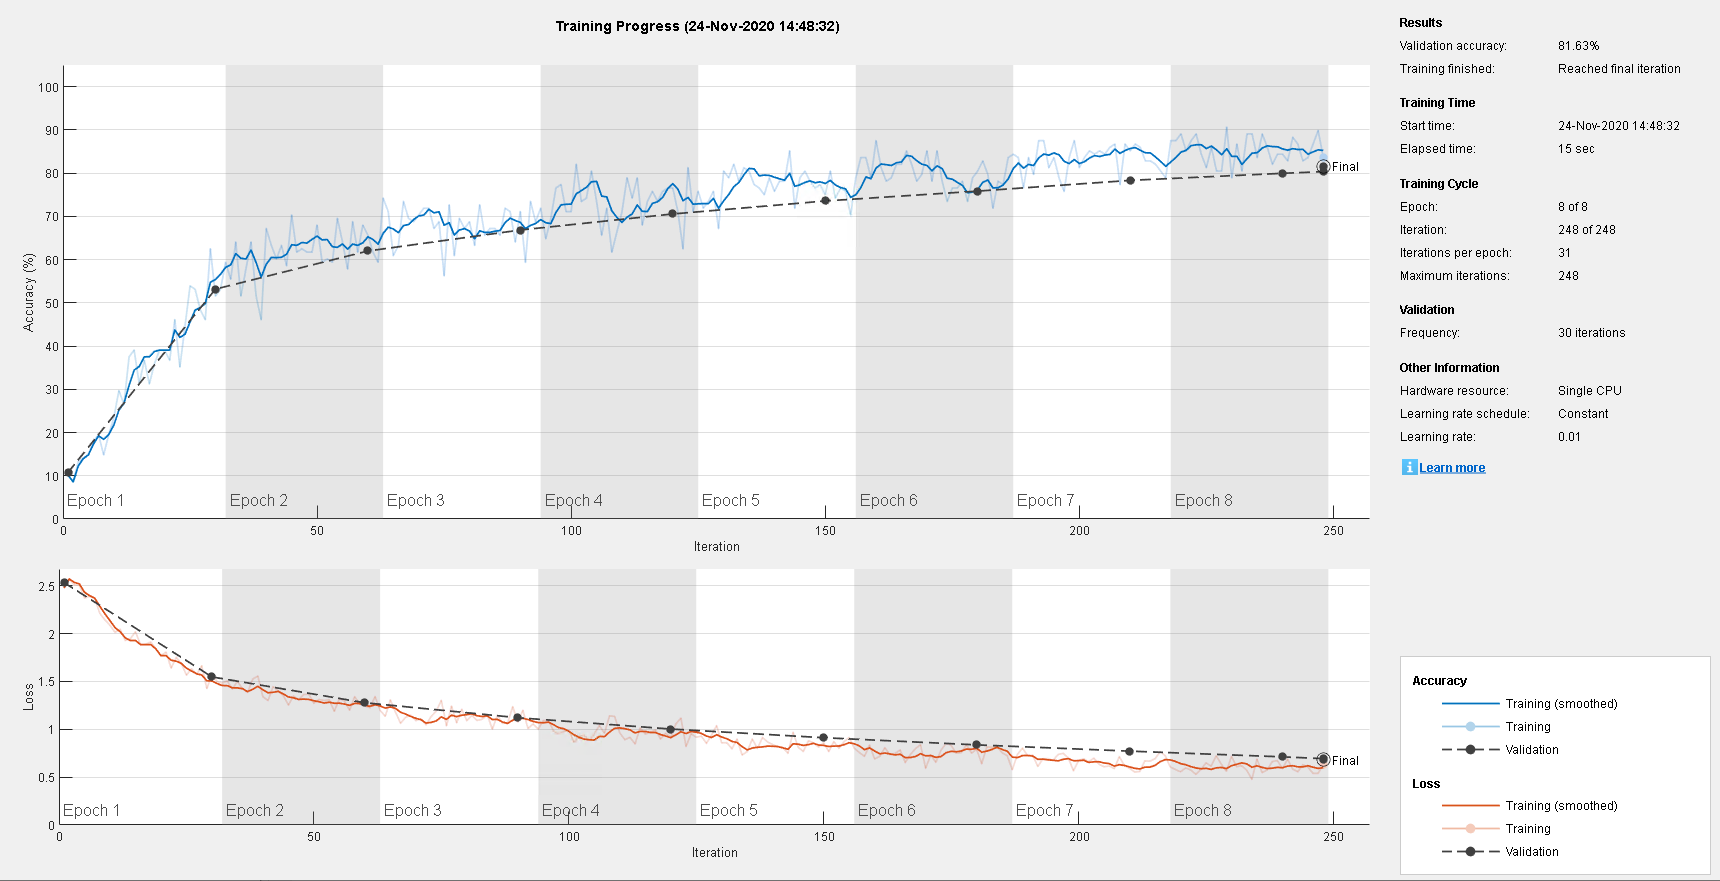
\includegraphics[width=1.24\textwidth]{fig-7f-040.png}}
    \caption{Curva di apprendimento: percentuale \emph{training}/\emph{validation} $0.4$.}
    \label{fig:04}
\end{figure}

\begin{figure}[htb]
    \vspace*{-1.2cm}\hspace*{-2.1cm}\framebox{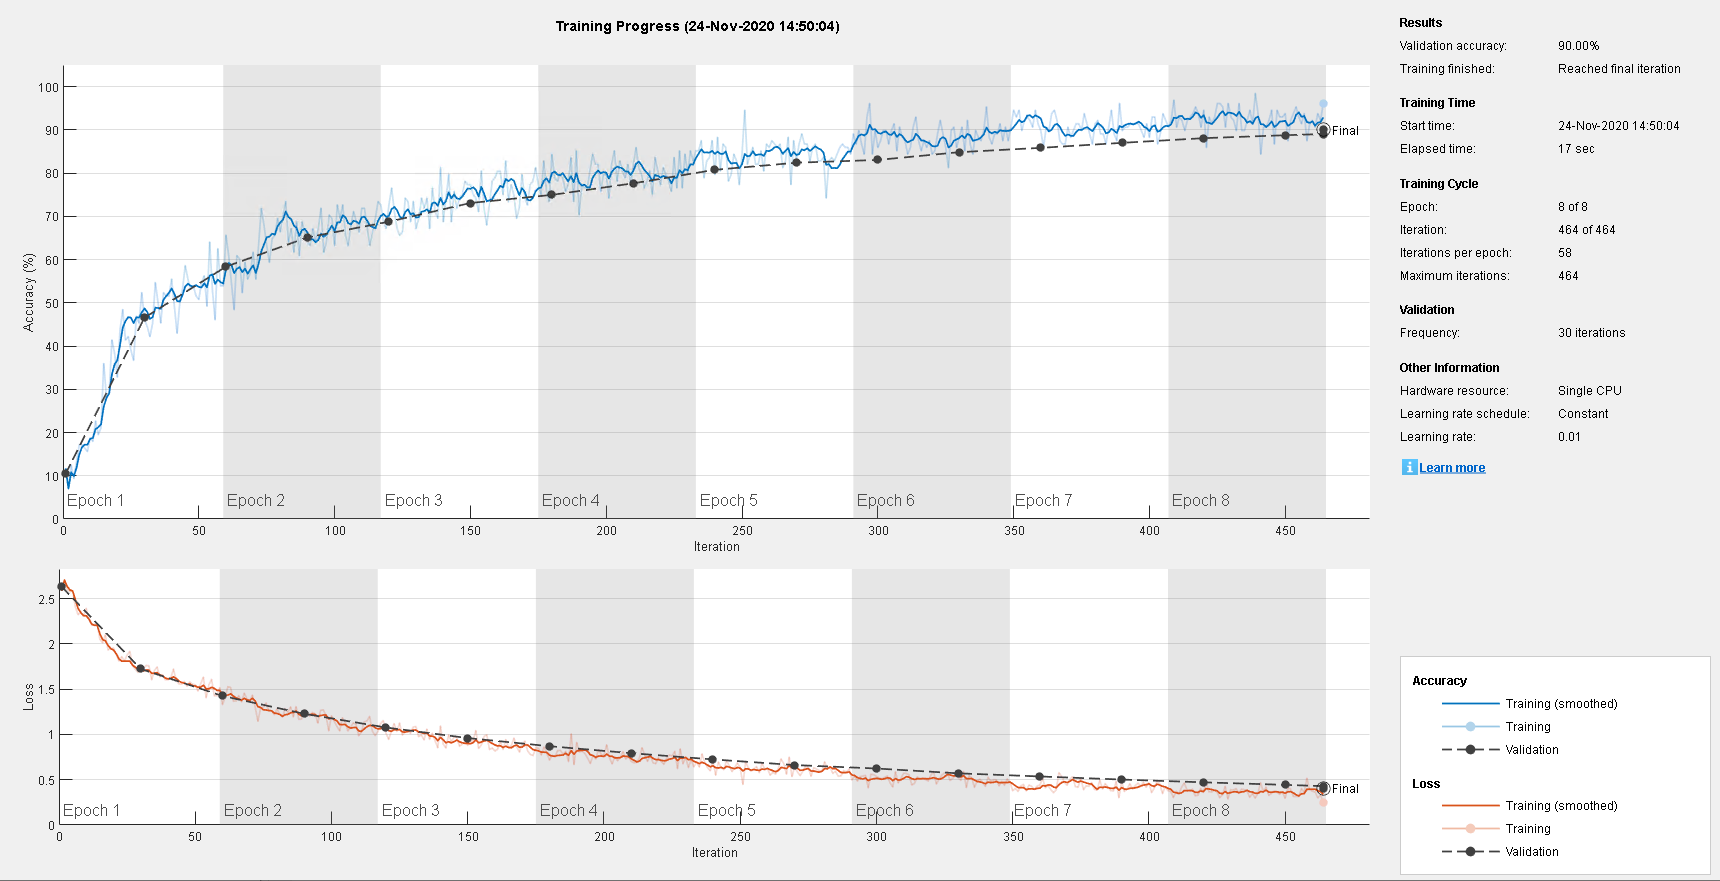
\includegraphics[width=1.24\textwidth]{fig-7f-075.png}}
    \caption{Curva di apprendimento: percentuale \emph{training}/\emph{validation} $0.75$.}
    \label{fig:075}
\end{figure}

\begin{figure}[htb]
    \hspace*{-2.1cm}\framebox{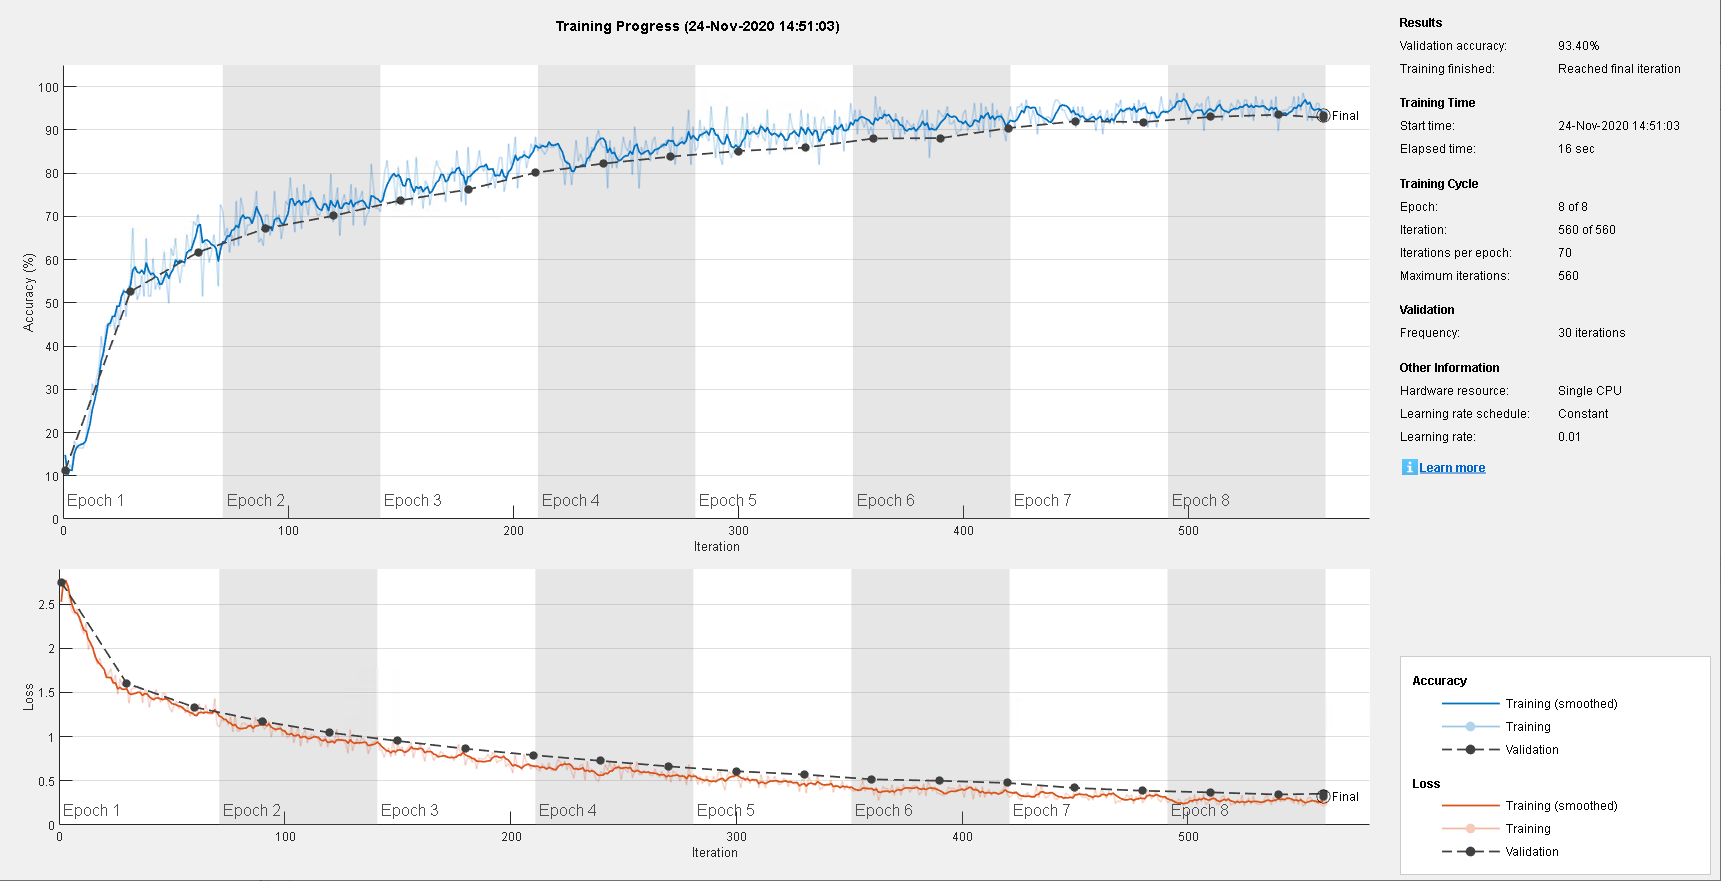
\includegraphics[width=1.24\textwidth]{fig-7f-090.png}}
    \caption{Curva di apprendimento: percentuale \emph{training}/\emph{validation} $0.9$.}
    \label{fig:09}
\end{figure}


\newpage ~ \newpage
\subsection{Curve di apprendimento al variare del numero di nodi nello strato nascosto}
Abbiamo modificato la struttura della rete cambiando il numero di nodi del livello nascosto: un \emph{hidden layer} da 10 nodi e uno da 50 nodi. Le curve di apprendimento risultanti sono riportate nelle Figure~\vref{fig:10} e~\vref{fig:50}.\medskip

Le \emph{validation accuracy} sono:
\begin{itemize}
    \item Strato nascosto da 10 nodi: $76.80\%$;
    \item Strato nascosto da 50 nodi: $94.00\%$.
\end{itemize}

\begin{figure}[htb]
    \hspace*{-2.1cm}\framebox{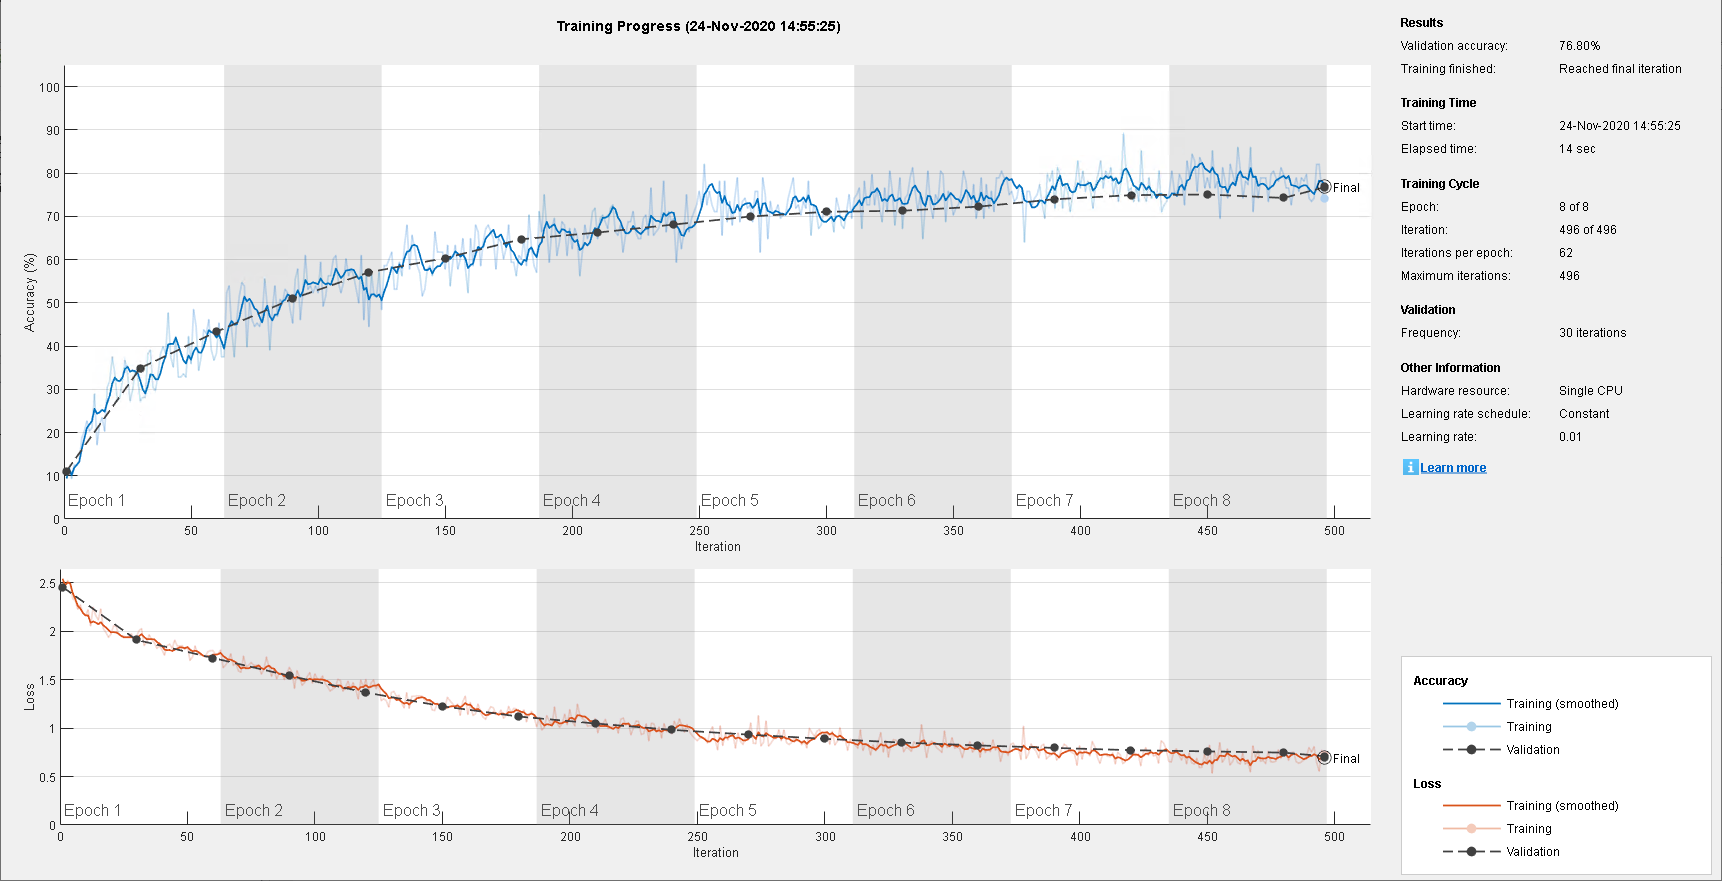
\includegraphics[width=1.24\textwidth]{fig-7g-10nodi.png}}
    \caption{Curva di apprendimento: 10 nodi nello strato nascosto.}
    \label{fig:10}
\end{figure}

\begin{figure}[htb]
    \hspace*{-2.1cm}\framebox{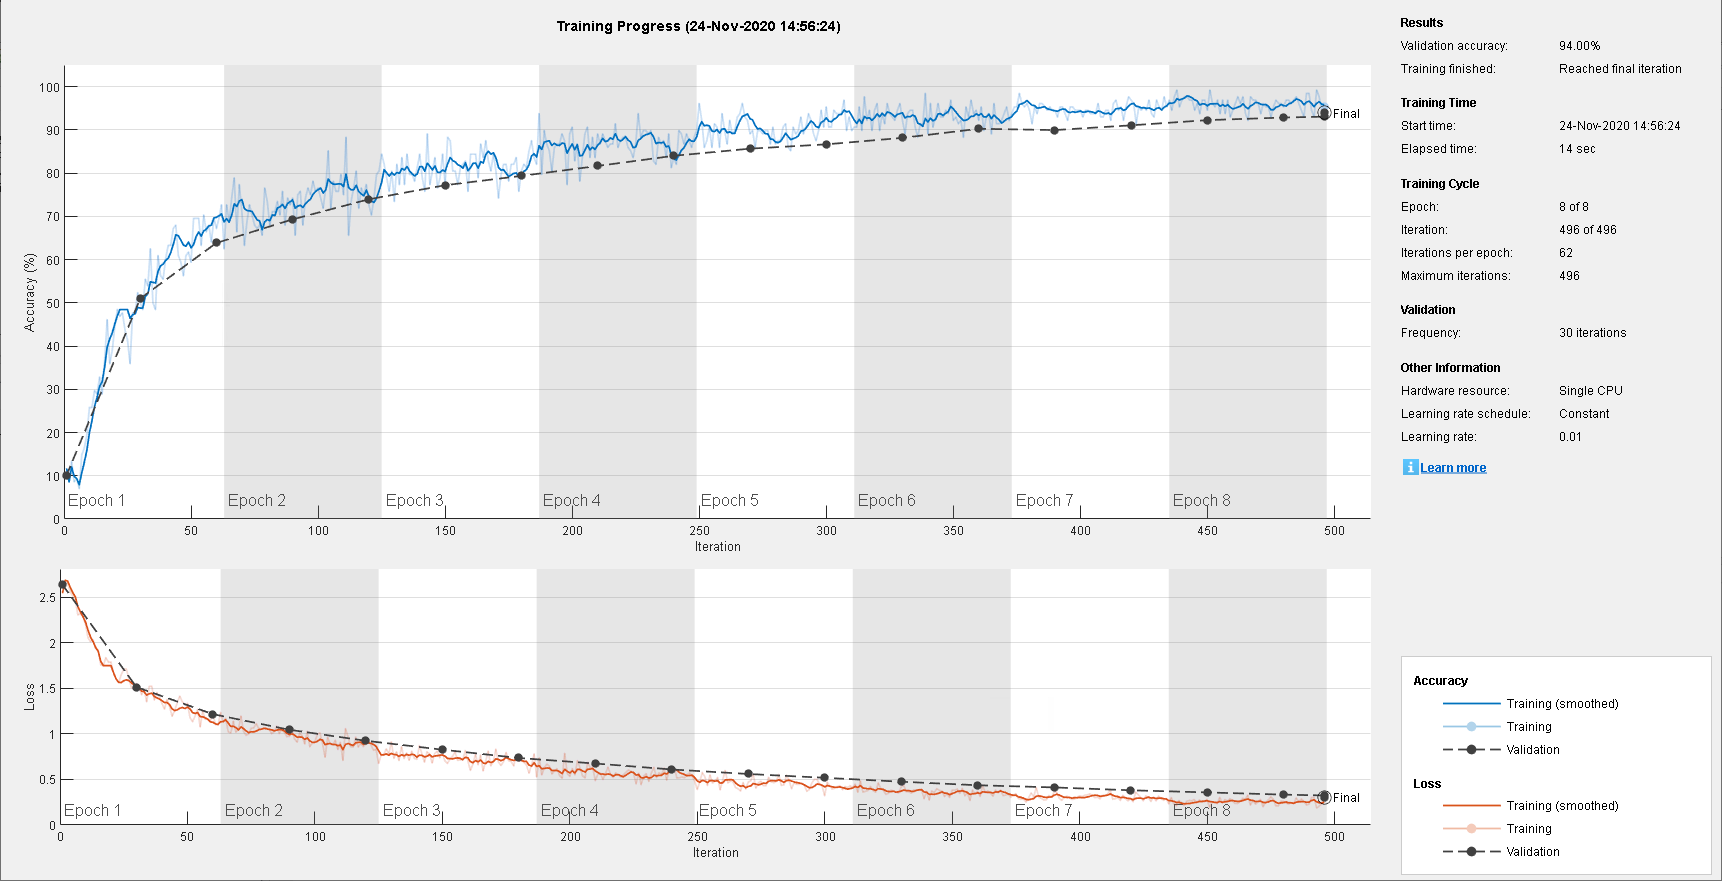
\includegraphics[width=1.24\textwidth]{fig-7g-50nodi.png}}
    \caption{Curva di apprendimento: 50 nodi nello strato nascosto.}
    \label{fig:50}
\end{figure}


\newpage ~ \newpage
\subsection{Modifica della rete e delle \emph{training options}: \emph{batch normalization layer} e \emph{stochastic gradient descent}}
Abbiamo modificato la struttura della rete omettendo lo strato \emph{batch normalization}. Abbiamo ripetuto l'addestramento sia con 8 epoche che con 80 epoche. Le curve risultanti sono riportate nelle Figure~\vref{fig:no-bn} e~\vref{fig:no-bn-80-epoch}.\medskip

Le \emph{validation accuracy} sono:
\begin{itemize}
    \item Rete senza \emph{batch normalization layer}, 8 epoche: $11.80\%$;
    \item Rete senza \emph{batch normalization layer}, 80 epoche: $16.60\%$.
\end{itemize}

\begin{figure}[htb]
    \hspace*{-2.1cm}\framebox{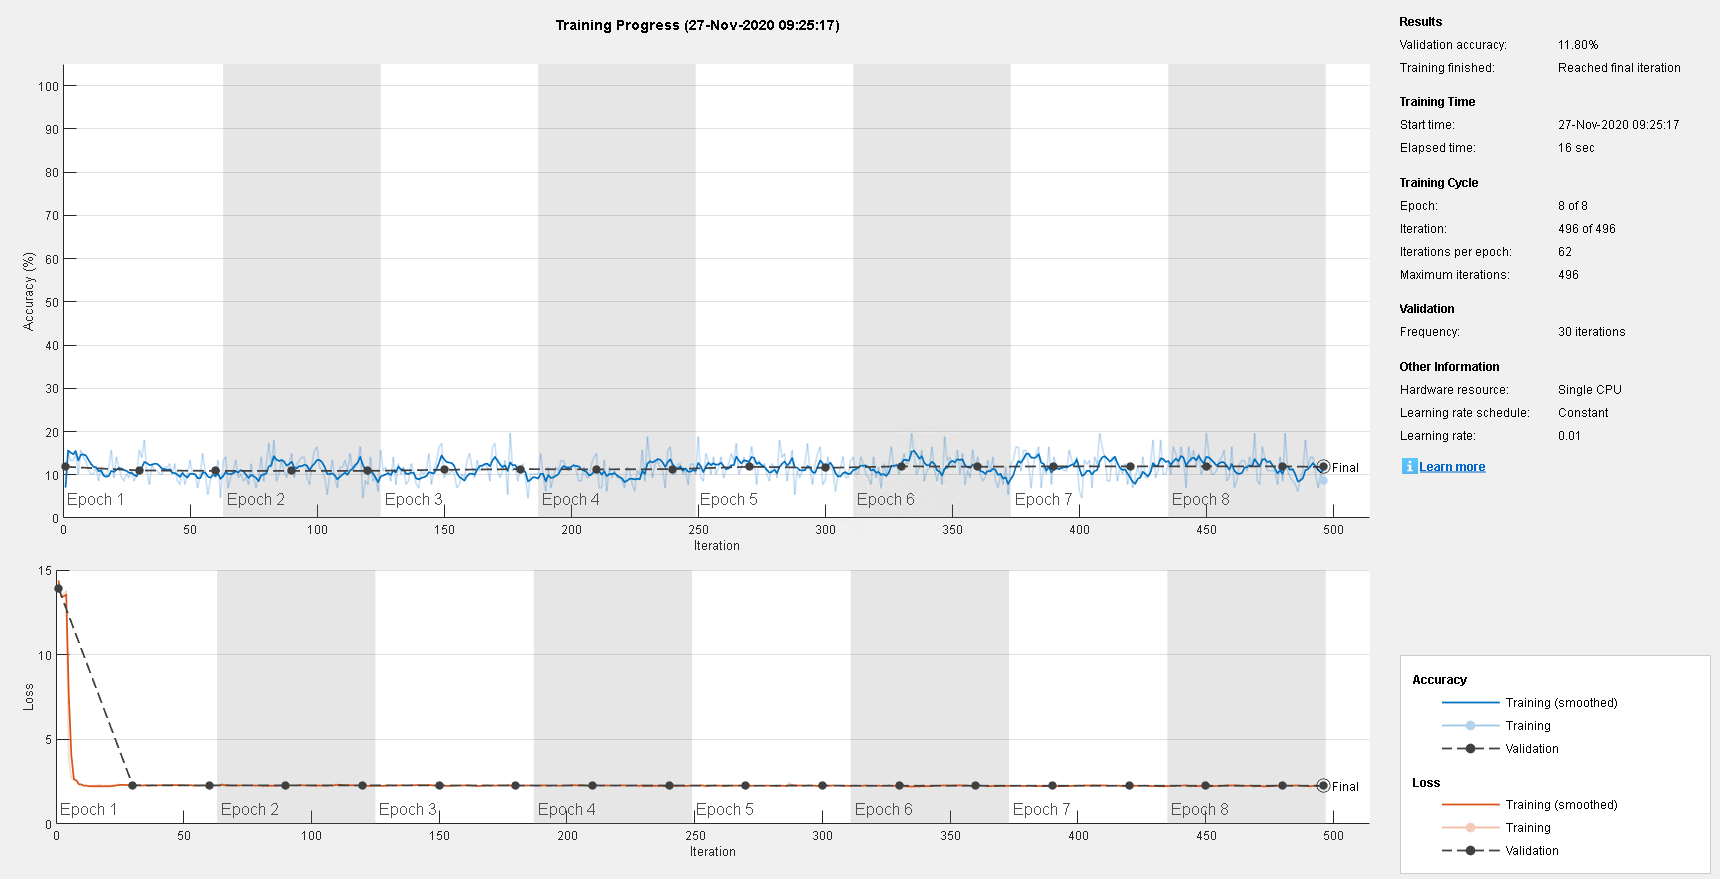
\includegraphics[width=1.24\textwidth]{senza-batchnorm.png}}
    \caption{Curva di apprendimento: rete senza \emph{batch normalization layer}.}
    \label{fig:no-bn}
\end{figure}

\begin{figure}[htb]
    \hspace*{-2.1cm}\framebox{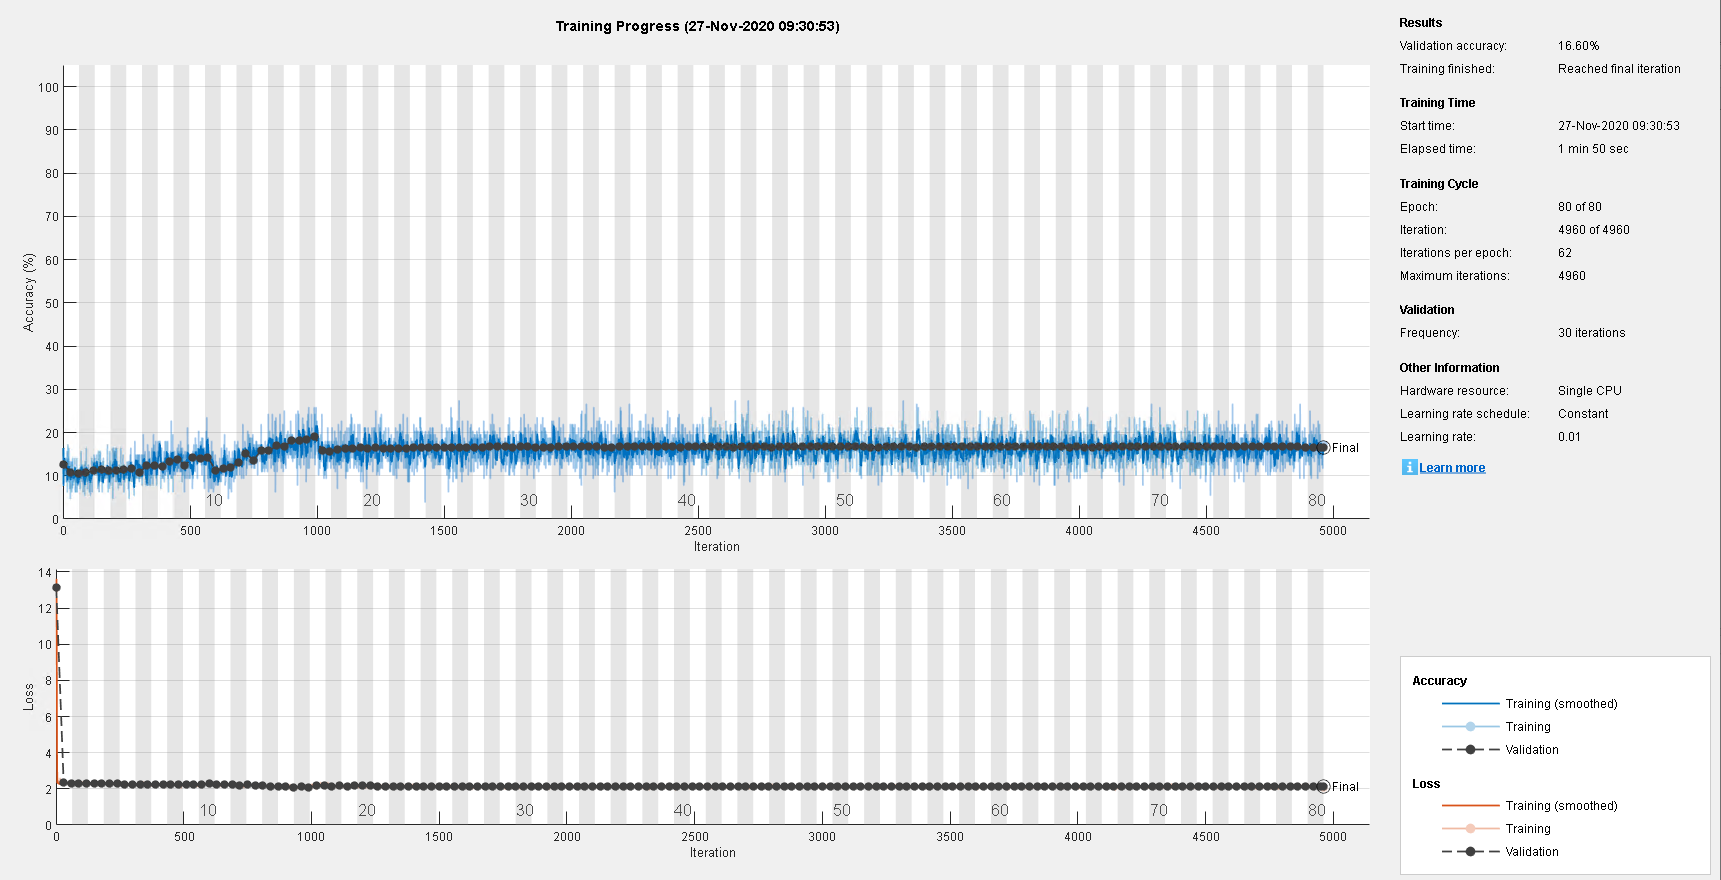
\includegraphics[width=1.24\textwidth]{senza-batchnorm-80epoche.png}}
    \caption{Curva di apprendimento: rete senza \emph{batch normalization layer}, 80 epoche.}
    \label{fig:no-bn-80-epoch}
\end{figure}

\newpage ~ \newpage
Abbiamo inoltre modificato le \emph{training options} utilizzando l'algoritmo di \emph{stochastic gradient descent} puro, senza \emph{momentum}. È stato sufficiente aggiungere la riga \texttt{'Momentum',0} alle opzioni. La curva risultante dall'addestramento della rete con queste modifiche si può vedere in Figura~\vref{fig:sgd}.

La \emph{validation accuracy} è, in questo caso, pari a $63.20\%$.


\begin{figure}[htb]
    \hspace*{-2.1cm}\framebox{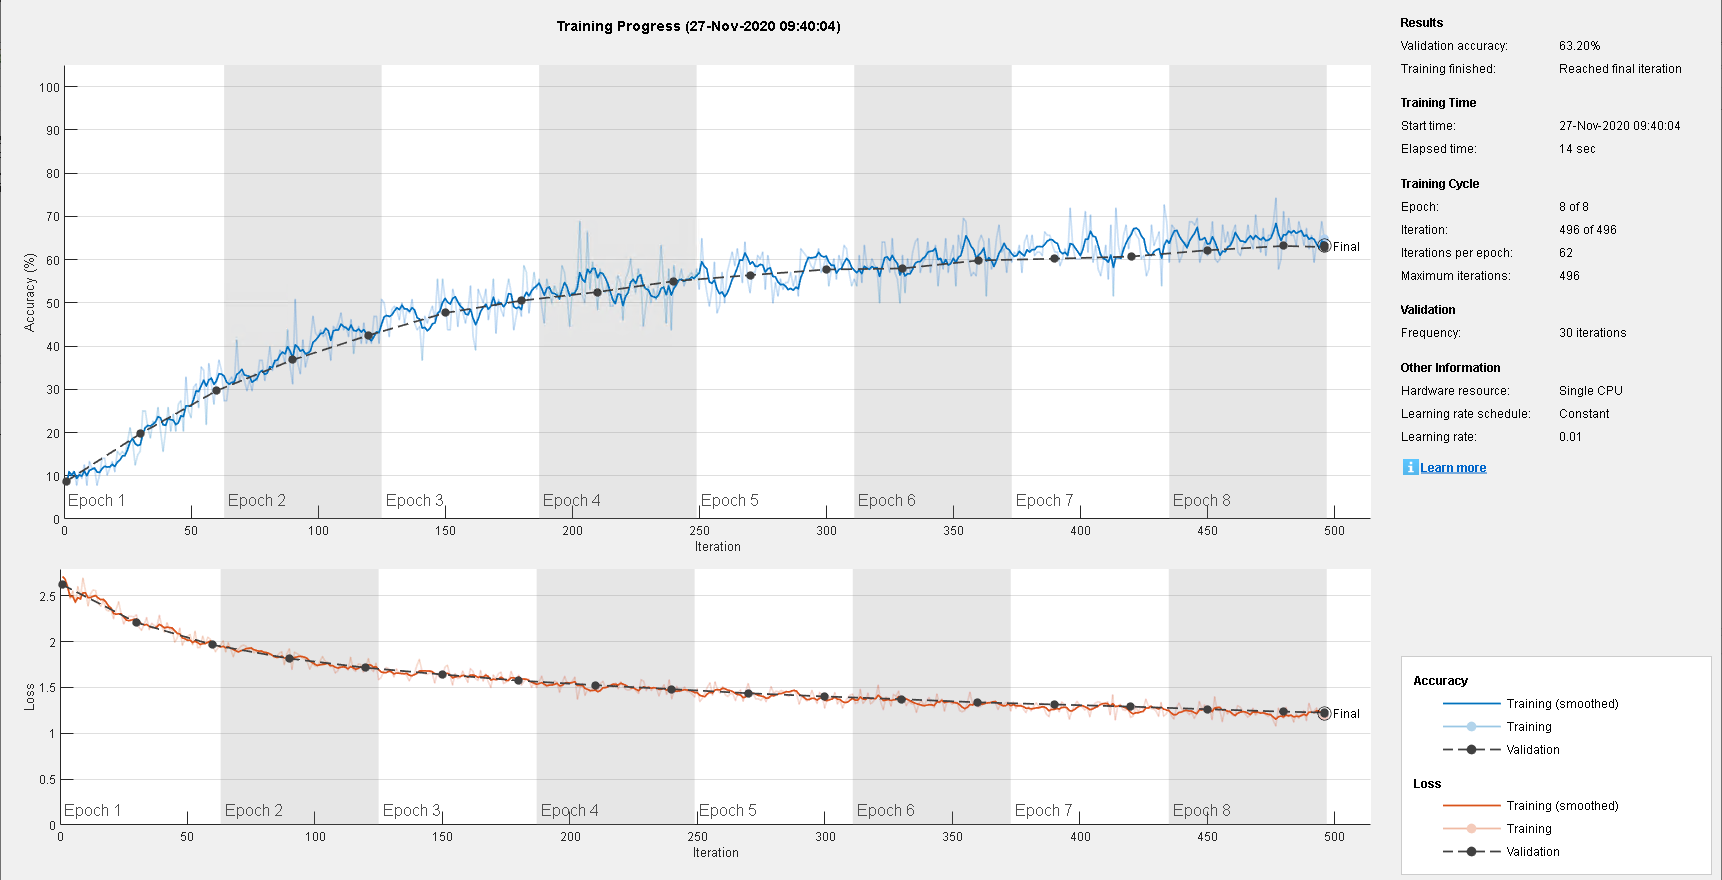
\includegraphics[width=1.24\textwidth]{sgd-momentum-0.png}}
    \caption{Curva di apprendimento che utilizza l'algoritmo SGD (senza \emph{momentum}).}
    \label{fig:sgd}
\end{figure}




\newpage
%%%%%%%%%%%%%%%%%%%%%%%%%%%%%%
\section{Osservazioni e Conclusioni} % cap8

Nel \textbf{secondo capitolo} abbiamo presentato il modello e l'architettura di rete. Nel \textbf{terzo capitolo} abbiamo illustrato come abbiamo preparato i dati strutturando gli insiemi di \emph{training} e di \emph{validation}. A seguire, nel \textbf{quarto capitolo} abbiamo presentato la struttura del software, che è articolato in due moduli.\medskip

Nel \textbf{quinto capitolo} abbiamo presentato il codice della funzione \texttt{MNIST\_DataPrep}. Si possono fare delle osservazioni sulla Figura~\vref{fig:a3} che mostra 20 immagini estratte a caso dal dataset MNIST. Oltre ad essere 20 immagini \emph{random}, ovvero scelte in maniera casuale tra le 10 000 immagini che compongono il dataset, si nota come siano presenti anche dei fenomeni di rotazione. Non tutte le cifre sono ``dritte'', ma alcune sembrano essere scritte al contrario, o di lato, o girate ad una certa angolazione.\medskip

Nel \textbf{sesto capitolo} abbiamo illustrato il codice dello script \texttt{MNIST\_Training}, che si occupa di definire l'architettura della rete, eseguire la fase di apprendimento, e analizzare le prestazioni della rete.\medskip

Nel \textbf{settimo capitolo} abbiamo presentato i risultati, che verranno qui discussi in dettaglio:

\paragraph{7.1 Curva di apprendimento della rete.} Il grafico dell'apprendimento è organizzato nel seguente modo:
\begin{itemize}
    \item Sull'asse delle ascisse c'è una distinzione tra \emph{iteration} e \emph{epoch}. La \emph{iteration} è una scansione di tutti gli input. In ogni epoca (8 in totale, come specificato nelle opzioni) vengono compiute 62 iterazioni: il numero totale di iterazioni è $62\times8=496$; 
    \item Nella parte superiore è riportata la curva blu relativa all'accuratezza. l'\emph{accuracy} è il numero di volte in cui ha successo la classificazione rispetto al numero totale di prove, quindi piu il suo valore è alto, migliore è il risultato. Osservando la curva in blu chiaro si notano delle fluttuazioni, l'accuratezza aumenta e diminuisce ad ogni passo. Queste fluttuazioni sono dovute alle incertezze statistiche di cui soffre l'accuratezza. Per ridurre le fluttuazioni viene fatto uno \emph{smoothing} (curva blu scuro): ogni 3 valori viene calcolata la media;
    \item La parte inferiore (curva rossa) è riferita alla \emph{loss} (\emph{cross entropy}). Anche in questo caso la curva più scura è quella in cui viene eseguito lo \emph{smoothing}. Osserviamo che, come ci aspettavamo, la curva \emph{cross entropy loss} diminuisce ad ogni passo;
    \item La curva nera è la curva di validazione.
\end{itemize}
Come già riportato, la \emph{validation accuracy} della rete neurale è $92.90\%$.


\paragraph{7.2 Validazione dell'apprendimento.} Utilizzando la rete addestrata, abbiamo predetto le etichette delle immagini nel \emph{validation set} per calcolare l'accuratezza della validazione finale. La \emph{accuracy} è la frazione di \emph{labels} che la rete classifica correttamente. In questo caso il $91\%$ (\emph{accuracy} = $0.9105$) delle etichette previste corrisponde alle etichette corrette del \emph{validation set}. 

Notiamo che la rete è la stessa del punto precedente, la cui \emph{accuracy} era del $92.90\%$. Questa piccola differenza tra i due valori è dovuta al fatto che si riferiscono a due addestramenti diversi. 


\paragraph{7.3 Curve di apprendimento al variare della percentuale di partizione del dataset.} Delle 10 000 immagini del dataset MNIST ne abbiamo dedicate finora l'$80\%$ al \emph{training set} e le restanti 2000 al \emph{validation set}. Abbiamo addestrato la rete cambiando questa proporzione: $40\%$, $75\%$ e $90\%$. Le \emph{accuracy} risultanti sono state rispettivamente dell'$81.63\%$, $90.00\%$ e $93.40\%$.

Osserviamo quindi come all'aumentare del numero di \emph{samples} dedicati al \emph{training set} aumenti anche l'accuratezza della rete, e quindi le sue prestazioni nel classificare correttamente le immagini.


\paragraph{7.4 Curve di apprendimento al variare del numero di nodi nello starto nascosto.} Lo strato nascosto della rete presenta 30 nodi. Abbiamo modificato questo strato diminuendone il numero a 10 ed aumentandolo a 50. I valori di \emph{accuracy} sono stati rispettivamente $76.80\%$ e $94.00\%$.

Nel caso della rete ``originale'' con 30 nodi l'accuratezza è stata calcolata attorno al $91-93\%$. Si osserva che mentre con uno strato nascosto con meno nodi (10) la \emph{accuracy} cala drasticamente, aggiungendone fino ad avere un \emph{hidden layer} di 50 nodi non aumenta di molto le prestazioni della rete.


\paragraph{7.5 Modifica della rete e delle \emph{training options}: \emph{batch normalization layer} e \emph{stochastic gradient descent}.} Togliendo lo strato di \emph{batch normalization}, l'accuratezza cala drasticamente da un valore superiore al $90\%$ a $11.80\%$. L'effetto permane anche aumentando il numero di epoche da 8 a 80: l'\emph{accuracy} in questo caso è del $16.60\%$.

Abbiamo utilizzato l'algoritmo \emph{stochastic gradient descent} settando a 0 il parametro \emph{mo\-men\-tum} nelle \emph{training options}. Da questa modifica si ottiene un'accuratezza del $63.20\%$.

Si può concludere che sia l'utilizzo del \emph{batch normalization layer} che dell'algoritmo di \emph{stochastic gradient descent with momentum} sono decisivi per un efficace addestramento della rete. In particolare, il \emph{batch normalization} è quantitativamente più decisivo.



\end{document}